\chapter{Dimensionality reduction of network epidiemiology
  model \label{ch:sis}}
% Abstract The exploration of epidemic dynamics on dynamically
% evolving (“adaptive”) networks poses nontrivial challenges to the
% modeler, such as the determination of a small number of informative
% statistics of the detailed network state (that is, a few “good
% observables”) that usefully summarize the overall (macroscopic,
% systems level) behavior. Trying to obtain reduced, small size
% accurate models in terms of these few statistical observables – that
% is, coarse-graining the full network epidemic model to a small but
% useful macroscopic one – is even more daunting. Here we describe a
% data-based approach to solving the first challenge: the detection of
% a few informative collective observables of the detailed epidemic
% dynamics. This will be accomplished through Diffusion Maps, a
% recently developed data-mining technique. We illustrate the approach
% through simulations of a simple mathematical model of epidemics on a
% network: a model known to exhibit complex temporal dynamics. We will
% discuss potential extensions of the approach, as well as possible
% shortcomings.

\section{Introduction}

Mathematical modeling of epidemic dynamics is an indispensable tool in
understanding and mitigating the spreading of disease in the real
world
\cite{gross_epidemic_2006,pastor-satorras_epidemic_2015,segbroeck_adaptive_2010,zhou_epidemic_2012}.
As computational power, numerical simulation techniques and, most
recently, “big data” tools and techniques progress, the degree of
realism in these mathematical models constantly improves. From simple
nonlinear models of Susceptible-Infected-Recovered (SIR) or
Susceptible-Infected-Susceptible (SIS) dynamics that are based on
spatial averaging (so called mean-field models, consisting of a few
nonlinear Ordinary Differential Equations (ODEs)) we have graduated to
models with detailed spatial information and structure, incorporating
not only geographical details of communities and cities but also
information about the social interactions between the individuals
involved
\cite{colizza_modeling_2006,wang_epidemic_2011,eubank_modelling_2004}.
From mean field ODEs the models now become large-scale, stochastic,
individual-based simulations on networks (geographical as well as
social).  While this framework is convenient for investigating many
different initial conditions combined with many different network
connectivities and many different interaction/evolution rules,
recording and rationalizing a useful summary of the dynamics (the
relevant macroscopic, systems-level statistics of these scenarios) is
crucial for systems-level understanding and control. Finding the right
macroscopic observables for such detailed simulations, the right
variables, to summarize the epidemic dynamics is still a daunting
task.

Over the last decade our group has proposed and developed the
so-called Equation-Free computational framework for complex/multiscale
systems modeling: given a detailed (here, individual/agent-based)
simulation algorithm, this framework enables the study of
coarse-grained, systems level dynamics through the design, execution
and processing of the brief bursts of fine scale simulation data;
Equation-Free algorithms like Coarse Projective Integration (CPI) take
the form of “wrappers” around the fine scale code (say, an agent-based
epidemic simulation code on an adaptive network)
\cite{gear_equation-free_2003,kevrekidis_equation-free:_2004,tsoumanis_coarse-graining_2012,siettos_equation-free_2011}. Yet
for this approach to be successful, one needs to a priori know what
the right macroscopic statistics are (e.g., the right few leading
moments of the distribution of susceptible or of infected individuals
in the population) in terms of which the epidemic statistics can be
informatively summarized.

This paper considers the case where such informative and parsimonious
system-level statistics are not a priori known.  In this case the
Equation-Free modeling approach can still be carried through, as long
as the right macroscopic variables can be discovered through the
mining of (big) computational simulation data. This is a
“doubly-data-based” modeling strategy: using data produced from
detailed, individual level, fine scale simulation bursts to detect the
number and identity of the macroscopic observables; and then, armed
with this knowledge, design and execute new, informative, microscale
simulations to systematically explore the evolution of the
epidemic. This jointly “equation-free, variable-free” approach holds
great promise for accurate, fast and informative systems-level
simulation of detailed, realistic epidemic models – the “right
observables” come from the (previously computed) data, as does the
design of “the right simulations” to obtain useful new information.


When the state of the fine-scale model at a given moment in time can
be mathematically described as a (long) vector in $\mathbb{R}^n$
(e.g. the state of a large number of agents), both linear data-mining
techniques, such as Principal Component Analysis (PCA), as well as
nonlinear data-mining techniques such as ISOMAP or Diffusion Maps
(DMAPS) can be applied to simulation data ensembles to obtain “the
right” macroscopic observables
\cite{jolliffe_principal_2014,coifman_diffusion_2006,tenenbaum_global_2000}. But
when the data involve evolving graphs (in our case, we are interested
in epidemic dynamics on adaptively evolving networks), finding good
macroscopic observables based on simulation databases is a nontrivial
task. We present a simple modification/extension of the DMAPS
procedure that allows us to detect the (small) number of these
observables for epidemics on adaptive networks based on data mining
only.  The “macro-variables” discovered by this process for the case
of a SIS epidemic on an adaptive network will be presented, discussed,
and contrasted to traditionally used macro-variables for the same
problem.

Our approach is motivated by, and illustrated through, SIS dynamics on
adaptive networks
\cite{gross_epidemic_2006,gross_adaptive_2008,gross_robust_2008}. The
computational methodology, however, is in principle applicable to many
problems that involve the dynamic evolution of networks with both
labeled nodes (when we know the identity of individuals) or unlabeled
nodes (when we do not)
\cite{sayama_modeling_2013,huepe_adaptive-network_2011}. We link the
DMAPS procedure with quantities that allow us to usefully compare
different networks; we use this approach to detect the number of
macroscopic observables involved in the dynamics of our SIS epidemic
model, and compare these data-based observables with typical network
statistics. The last few years have seen several innovative approaches
to finding accurate reduced models for dynamic, network-evolution
problems, extending and complementing well-established techniques like
those based on moment closures \cite{gross_robust_2008}. Our approach
should be considered as a data-mining based alternative to these
techniques with the advantages of not requiring any knowledge about
the underlying model and automating the process of feature extraction.

The rest of the paper is organized as follows: We will first describe
our implementation of a SIS epidemic model on an adaptive network,
from which the simulation data will be obtained. We then briefly
discuss established linear (PCA) and nonlinear (DMAPS) data mining
techniques. We then present an extension to DMAPS that expands their
applicability to data in the form of evolving networks (where the
connectivity of the network evolves in time along with the state of
the network nodes). We first validate our network data mining approach
on data obtained from a simple Watts-Strogatz network model
\cite{watts_collective_1998}. We then present our main results: the
application of our data-mining technique to data collected from
dynamic SIS simulations on an adaptive network, obtained over a range
of epidemic parameter values where it is known that complex,
oscillatory dynamics arise. We discuss the relation of the variables
detected through our approach to those of more traditional,
moment-based approaches, and conclude with a brief perspective on
potential shortcomings but also potential fruitful applications of the
approach.

\section{The adaptive SIS model}

An implementation of the adaptive SIS model can be constructed by
considering a labeled graph $G$ with $N$ nodes and $L$ links, with
each node representing an individual in a social network; the state of
each individual, either susceptible (S) or infected (I), constitutes
the node label. Edges between individuals are defined as SS-links,
II-links, or SI-links, according to the label of the nodes they
connect. Starting with a given initial network connectivity pattern (a
given network topology), the evolution of the model can be
characterized by three substeps, which together constitute a time step
in the model's evolution:

\begin{enumerate}
  \item All infected nodes recover with
    probability $r$, becoming susceptible.
  \item For every SI-link, the
    susceptible individual becomes infected with probability $p$.
  \item Every SI-link is removed with probability $w = w_0 \rho$. In this case, a
    new edge between the corresponding susceptible node and another
    susceptible node is formed. The new link is made with a node
    chosen uniformly at random from the set of all other susceptible
    individuals.
\end{enumerate}

The probability of rewiring $w = w_0 \rho$ is based on a constant
input parameter $w_0$ and the infected fraction $\rho = i/N$, where
$i$ is the number of infected nodes. These rules are motivated by the
assumption that humans are more likely to avoid infected individuals
proportionally to their awareness of disease spread, which here is
assumed to be directly proportional to the infected fraction of the
population \cite{gross_epidemic_2006}. Figure~\ref{fig:sis2} shows a
schematic of this evolution process, while Figure~\ref{fig:sis1} gives
a sense of the model behavior in different parameter regimes.

Although the behavior of this model is inherently complex (see the
bifurcation diagram in Figure~\ref{fig:sis1}, reproduced by
permission) \cite{gross_robust_2008}, it has been previously
established that the system-level dynamics of a sufficiently large
network can be captured by just three macroscopic observables: the
number of infected nodes $i$, the number of SS-links $l_{SS}$ and the
number of II-links $l_{II}$ . These variables suffice to describe all
long-term dynamical behavior exhibited by the system, since the values
of other variables (higher order moments of the network state) quickly
become slaved to (functions of) these three and do not contribute
extra degrees of freedom over long timescales. As the infection
parameter $p$ varies, one can observe stationary states as well as
coarsely oscillatory dynamics, and even coexistence between the two
(associated with an apparent subcritical coarse Hopf bifurcation)
\cite{holmes_turbulence_2012}.  In this paper we will show how to
extract the relevant observables responsible for the dynamics of the
system without making use of any prior knowledge about their
suitability. This will be accomplished by first constructing a
suitable similarity measure for quantifying graph differences, and
secondly, by applying DMAPS on ensembles of graphs resulting from the
dynamic simulation of the model’s evolution.

\begin{figure}[!htp]
\centering
\begin{tabular}{cc}
  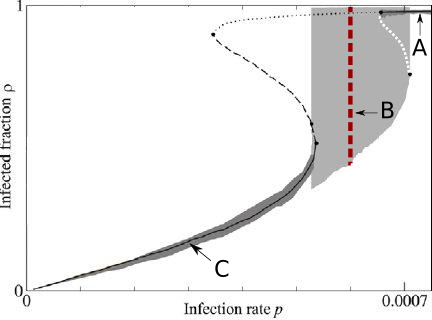
\includegraphics[width=0.45\textwidth]{1a} &
  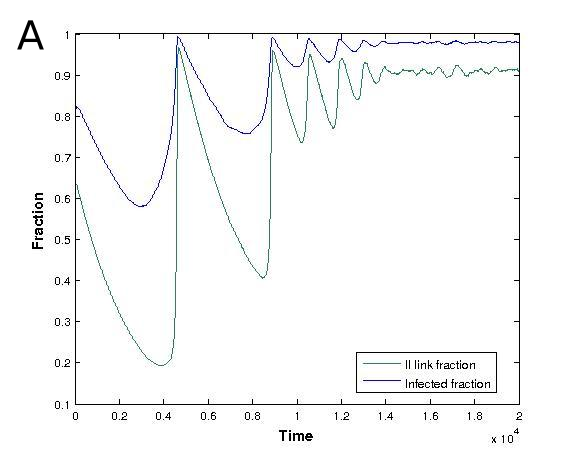
\includegraphics[width=0.45\textwidth]{1b}\\
  (a) & (b)\\
  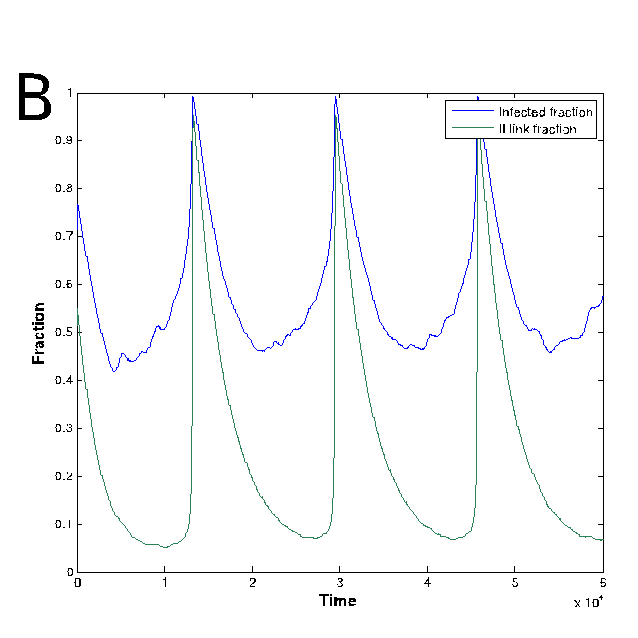
\includegraphics[width=0.45\textwidth]{1c} &
  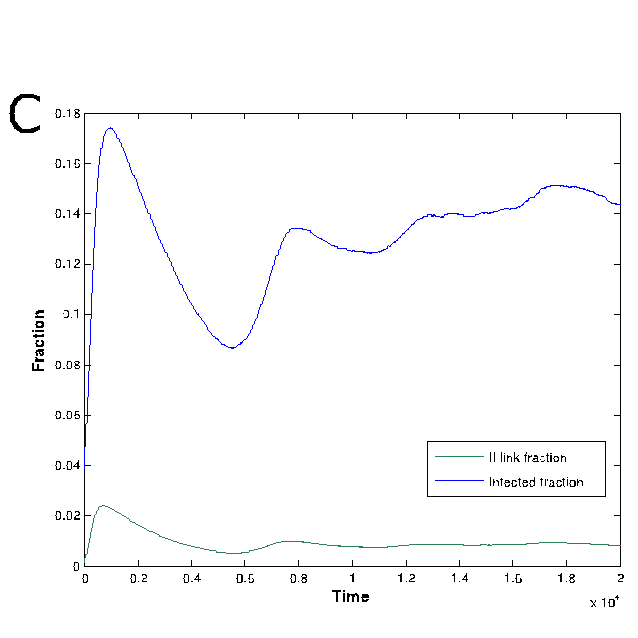
\includegraphics[width=0.45\textwidth]{1d}\\
  (c) & (d) \\
  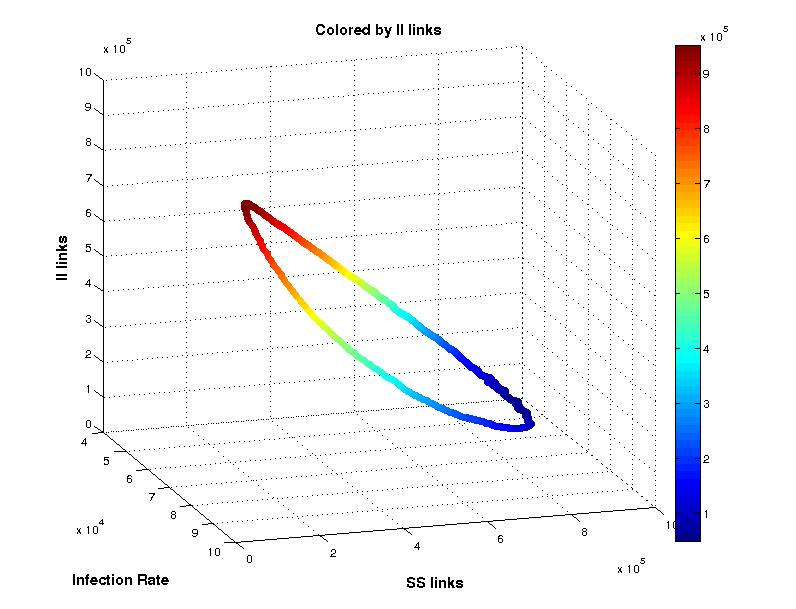
\includegraphics[width=0.45\textwidth]{1e} &
  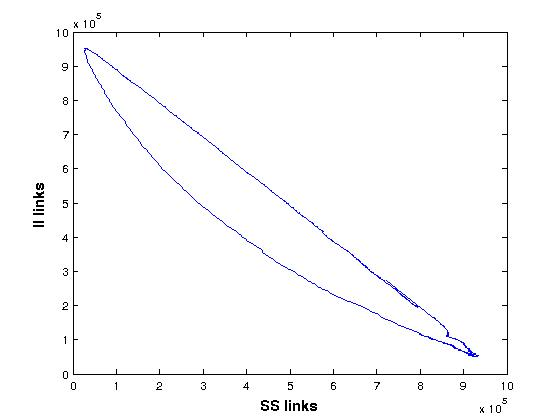
\includegraphics[width=0.45\textwidth]{1f}\\
  (e) & (f)
\end{tabular}
\caption{(a) Model bifurcation diagrams wrt. the infection rate
  parameter $p$ (reprinted with permission)
  \cite{gross_epidemic_2006}. (b) The system evolves to a stable
  stationary state for $p = 0.00073$. (c) Oscillatory behavior
  indicating a (coarse) limit cycle at $p = 0.0006$. (d) Stable
  stationary state for $p = 0.0003$. Bottom graphs indicate the
  relationship between $i$, $l_{SS}$ , and $l_{II}$ over the course of
  one complete oscillation for $p = 0.0006$. Model parameters:
  $(r, w_0, N, L) = (0.0002, 0.03, 10^5 , 10^6)$. \label{fig:sis1}}
\end{figure}

\begin{figure}[!htp]
\centering
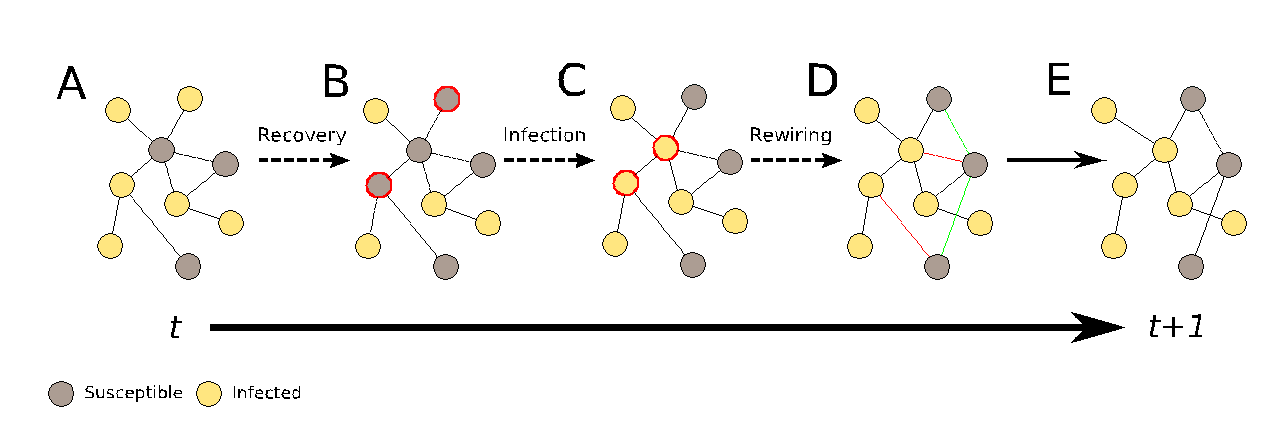
\includegraphics[width=0.9\textwidth]{2}
\caption{Schematic of the adaptive SIS model evolution: the three
  substeps constituting one SIS evolution timestep. (A) The initial
  graph at time $t$. (B) Each infected node recovers with probability
  $r$, becoming susceptible. (C) The disease spreads along SI-links
  with probability $p$, infecting susceptible nodes. (D) With
  probability $w$, each SI-link is broken and a new SS-link is
  created. (E) The final graph at $t+1$. Broken links and nodes that
  change status between steps are colored in red, while rewired links
  are colored in green. \label{fig:sis2}}
\end{figure}

\section{A brief discussion of dimensionality reduction}

Analysis of the dynamics of this epidemic model, especially as the
size of the network grows, is hindered by its size and complexity. Not
only are there many nodes to keep track of over thousands of time
steps, but each step is also comprised of a number of different
(stochastic) actions. These factors combine to make systematic
exploration of such a system computationally intractable; one may only
execute and observe many different scenarios computationally
(different initial networks, node states, and parameter
values). Additionally, it is not clear which variables, or indeed even
how many, play a determining role in summarizing long-term system
behavior. This motivates the development of an algorithmic approach to
identifying the crucial features of the system. Not only will these
important features themselves aid in better understanding the problem
and in summarizing its behavior, but they could also be used in an
Equation-Free framework to enable the sort of analysis typically
reserved for simpler systems (e.g. a few mean-field ODEs). Below, we
present our first step towards this goal: the use of the DMAPS data
mining technique to identify the important observables in the SIS
model from simulation datasets.

\section{Principal component analysis and diffusion maps}

Given a dataset ${x_1, x_2, \dots, x_N}$ (with each
$x_i \in \mathbb{R}^n$), several approaches exist to uncover a
lower-dimensional description ${y_1, y_2, \dots, y_N}$ of the data,
where $y_i \in \mathbb{R}^p$ and $p \ll n$. These new
lower-dimensional points $y_i$ accurately capture the salient features
of the original data set, with minimal loss of important
information. In essence, we try to describe our data as concisely as
possible.

Perhaps the best-known method for achieving this is Principal
Component Analysis (PCA) \cite{jolliffe_principal_2014}, detailed in
Section~\ref{sec:ml:pca}. Unfortunately, PCA assumes the data lies on,
or around, a linear subspace, whereas data points generally lie on
nonlinear manifolds. To circumvent this limitation we turn to the
nonlinear dimensionality reduction technique of Diffusion Maps (DMAPS)
\cite{coifman_diffusion_2006}. The algorithm is detailed in
Section~\ref{sec:dmaps}. In brief, by simulating a diffusion process
over the dataset, DMAPS will reveal the underlying low-dimensional
nonlinear structure.

\section{Similarities between different networks}

In order to simulate diffusion over the dataset, DMAPS requires a
scalar distance between two data points, $d(x_i, x_j)$. When each
point is a vector the Euclidean distance between points is often
sufficient. However, in the dataset we investigate below, each point
$x_i$ is not a vector, but actually a graph (or network), which we
represent as $G_i$.

The literature contains a number of ways of quantifying the distance
between two graphs, $d(G_i, G_j)$, for example by measuring how easily
$G_i$ can be transformed into $G_j$ (graph edit distance), or by
comparing random walks on the graphs (spectral distance)
\cite{bunke_graph_1998,gao_survey_2010,papadimitriou_web_2010,vishwanathan_graph_2010}. In
this paper, we consider two graphs to be similar if they share similar
numbers of certain features. More precisely, we define a list of $k$
subgraphs $S = {s_1, s_2, \dots, s_k}$, such as the single edge, the
two connected edges, the triangle shown in Figure~\ref{fig:sis4} etc. Then we
record how many times each subgraph appears in our input graph in a
vector $v_i = {c_1^i, c_2^i, \dots, c_k^i}$, where $c_j^i$ is the
number of times subgraph $s_j$ was found in input graph $G_i$. This
process maps each graph to a vector of subgraph densities, the counts
$G_i \rightarrow v_i, \; v_i = {c_1^i, c_2^i, \dots, c_k^i}$ in
$\mathbb{R}^k$, thus embedding the graph as a point in
$\mathbb{R}^k$. We then use these k-long vectors (k-dimensional
points) as the input to DMAPS, and use the Euclidean distance between
them as our notion of graph similarity. Thus
$d(G_i, G_j) = \| v_i - v_j \|_2$. Figure~\ref{fig:sis4} presents a schematic
illustrating this subgraph-enumeration process.


In the SIS model, we are actually working with labeled graphs, since
each node has one of two labels – susceptible (S) or infected (I). It
is inappropriate to simply ignore network labels, since networks with
the same connectivity, but with different node labels, can behave in
extremely different ways and should thus be considered dissimilar. To
overcome this issue, for a given labeled graph $G$ we choose to
consider three separate unlabeled subgraphs $G_0, G_S$ and $G_I$. Here
$G_0$ is the initial graph $G$ without node labels and $G_S$, $G_I$
the unlabeled subgraphs obtained (induced) by only considering the S,
or the I nodes respectively. We will represent each overall labeled
graph by the concatenation of the three count vectors $v_0, v_I, v_S$
into $v = [v_0 v_I v_S]^T$, again using the Euclidian norm to quantify (dis)similarity
between them. Note that we scale the subgraph counts so that we really
measure a “density” of $s$ in $G$, given by:

\begin{align}
  \label{eqn:homdenG}
  \rho(H,G) := \frac{1}{{n\choose k}} \!  \sum_{\varphi:[k] \to [n]} \!
  \left[ \forall  i, j \in [k] \! : \! H(i,j) \! = \! G(\varphi(i),
  \varphi(j)) \right].
\end{align}

where $n$ is the number of nodes in $G$, $k$ is the number of nodes in
$s$, $\varphi$ is an injection from the first $k$ integers to the
first $n$, and $\!$ is an indicator function which takes the value 1
when subgraph $s$ has been located in $G$. The subgraph enumeration
procedure in the case of labeled nodes is illustrated in Figure~\ref{fig:sis5}.

\begin{figure}[!htp]
\centering
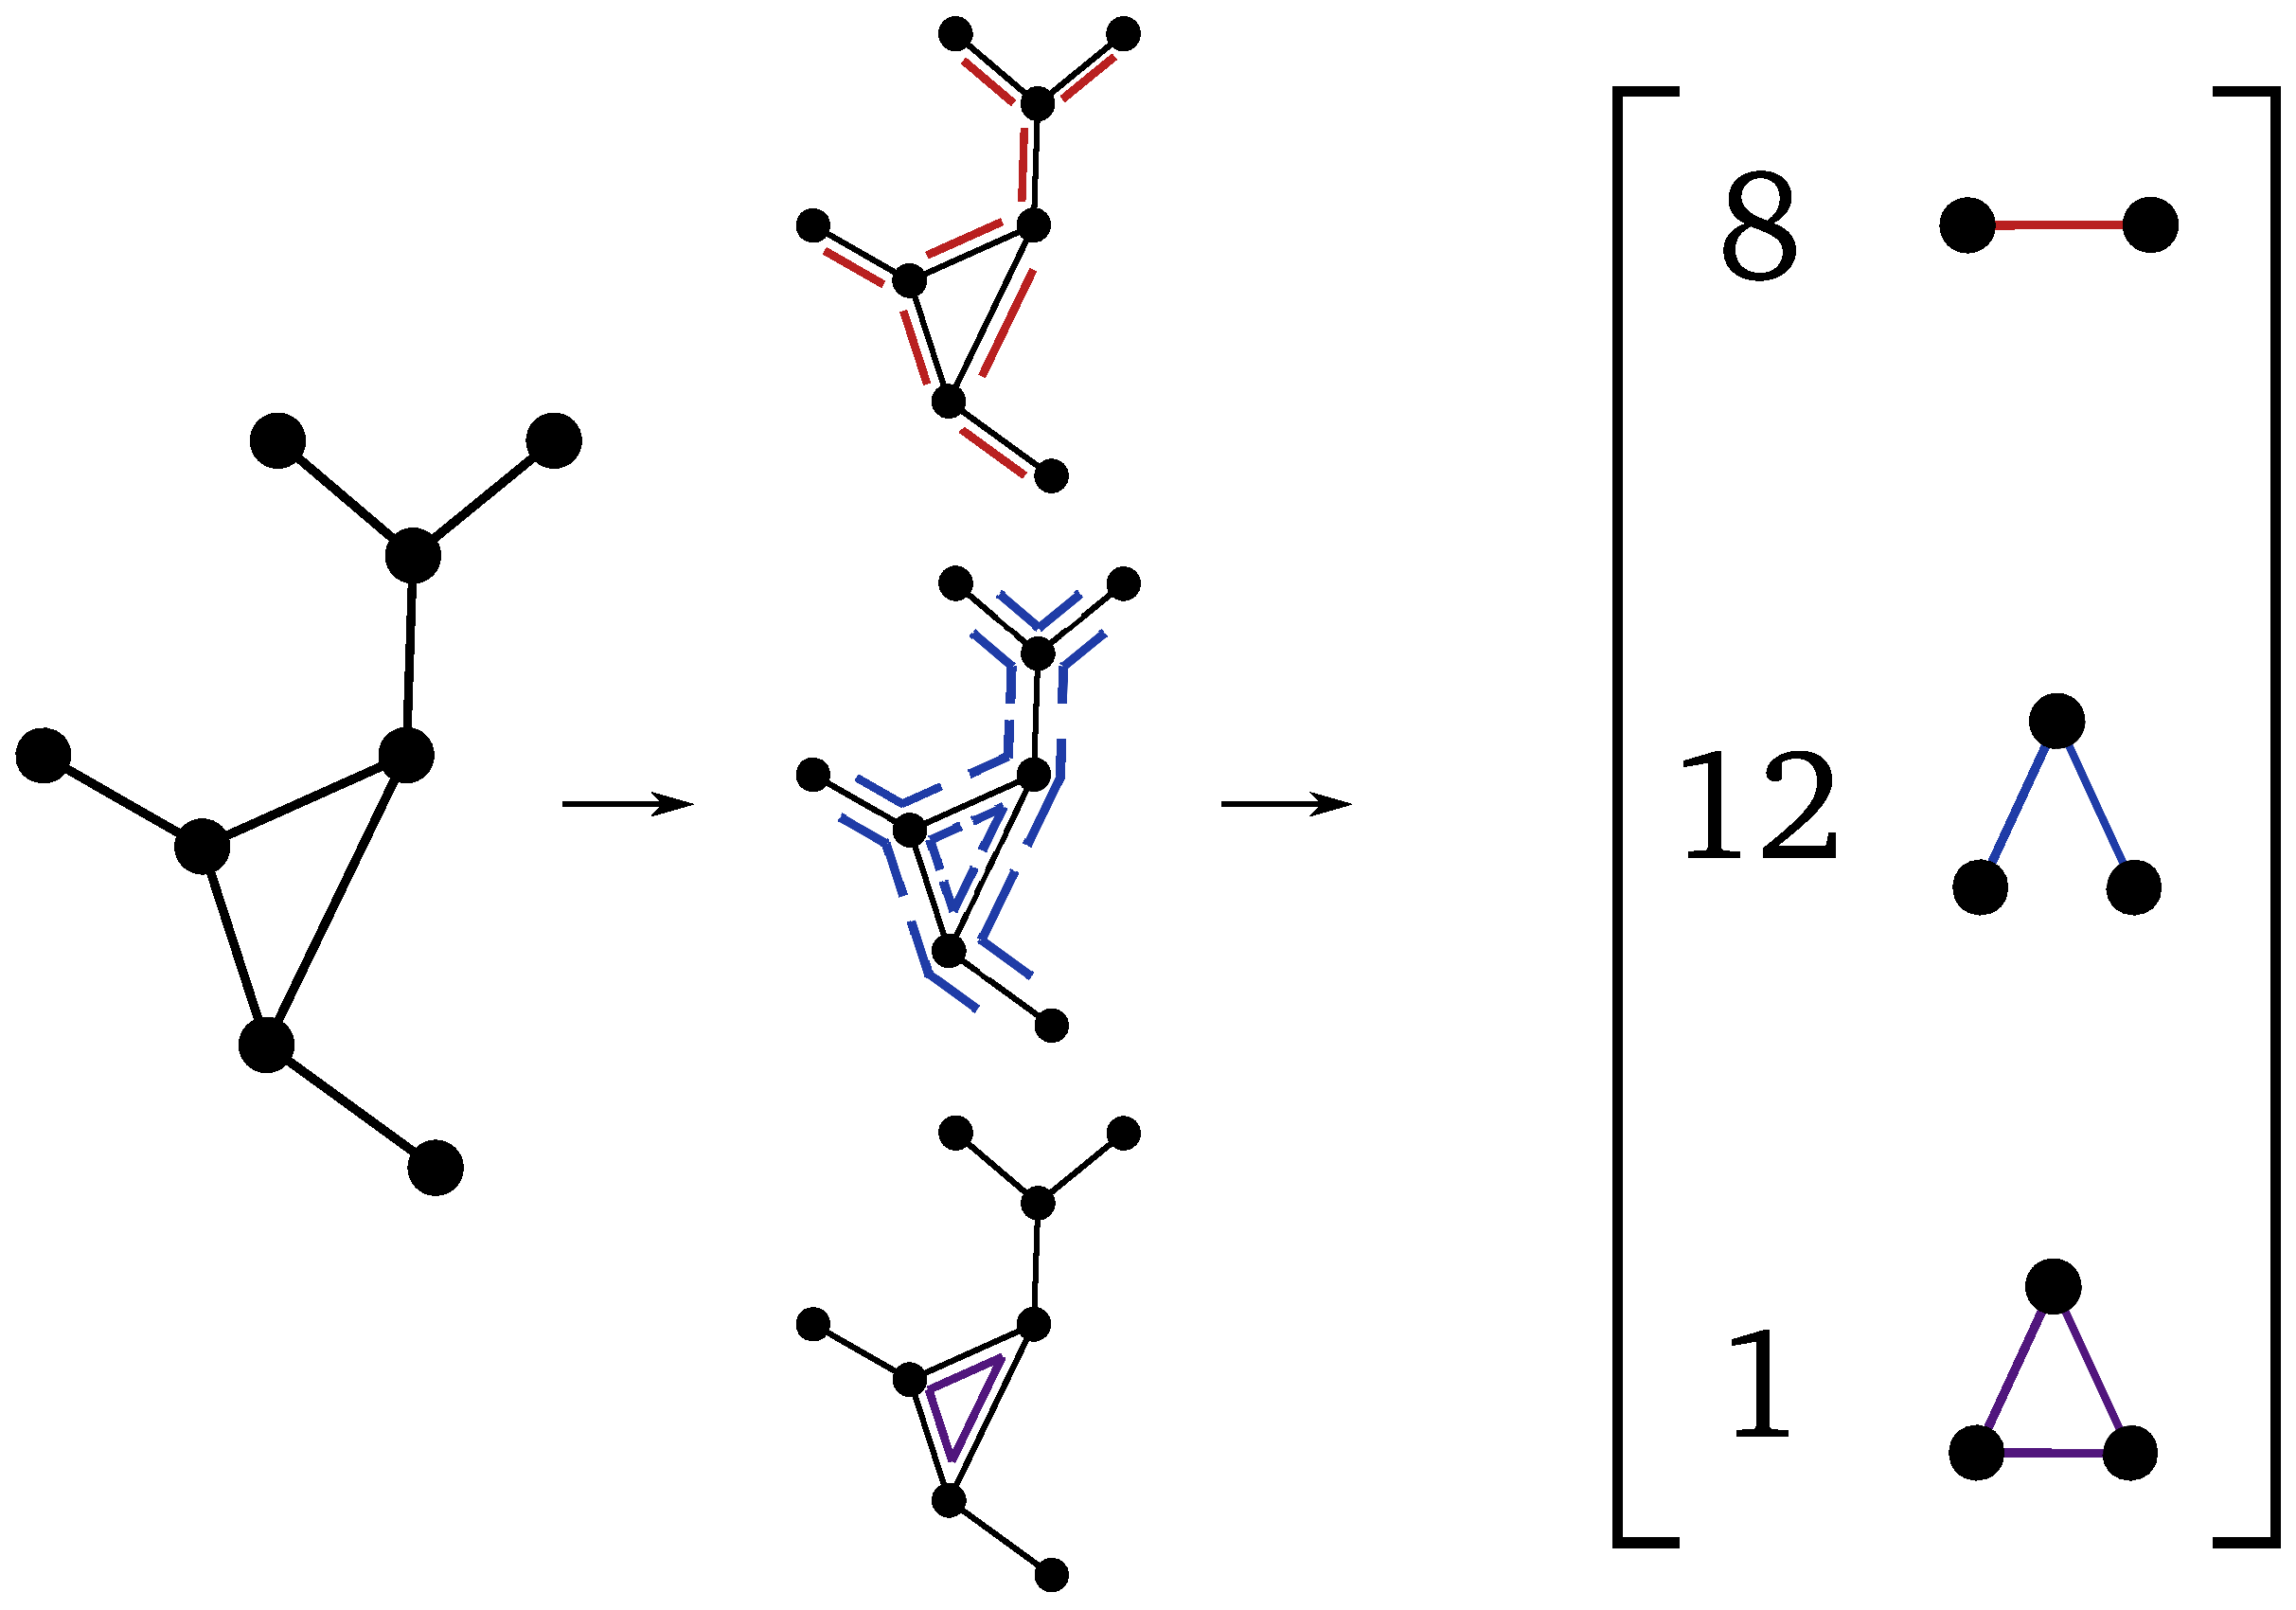
\includegraphics[width=0.9\textwidth]{subgraph-counting}
\caption{Illustration of the subgraph-enumeration process with an
  unlabeled input graph. \label{fig:sis4}}
\end{figure}

\begin{figure}[!htp]
\centering
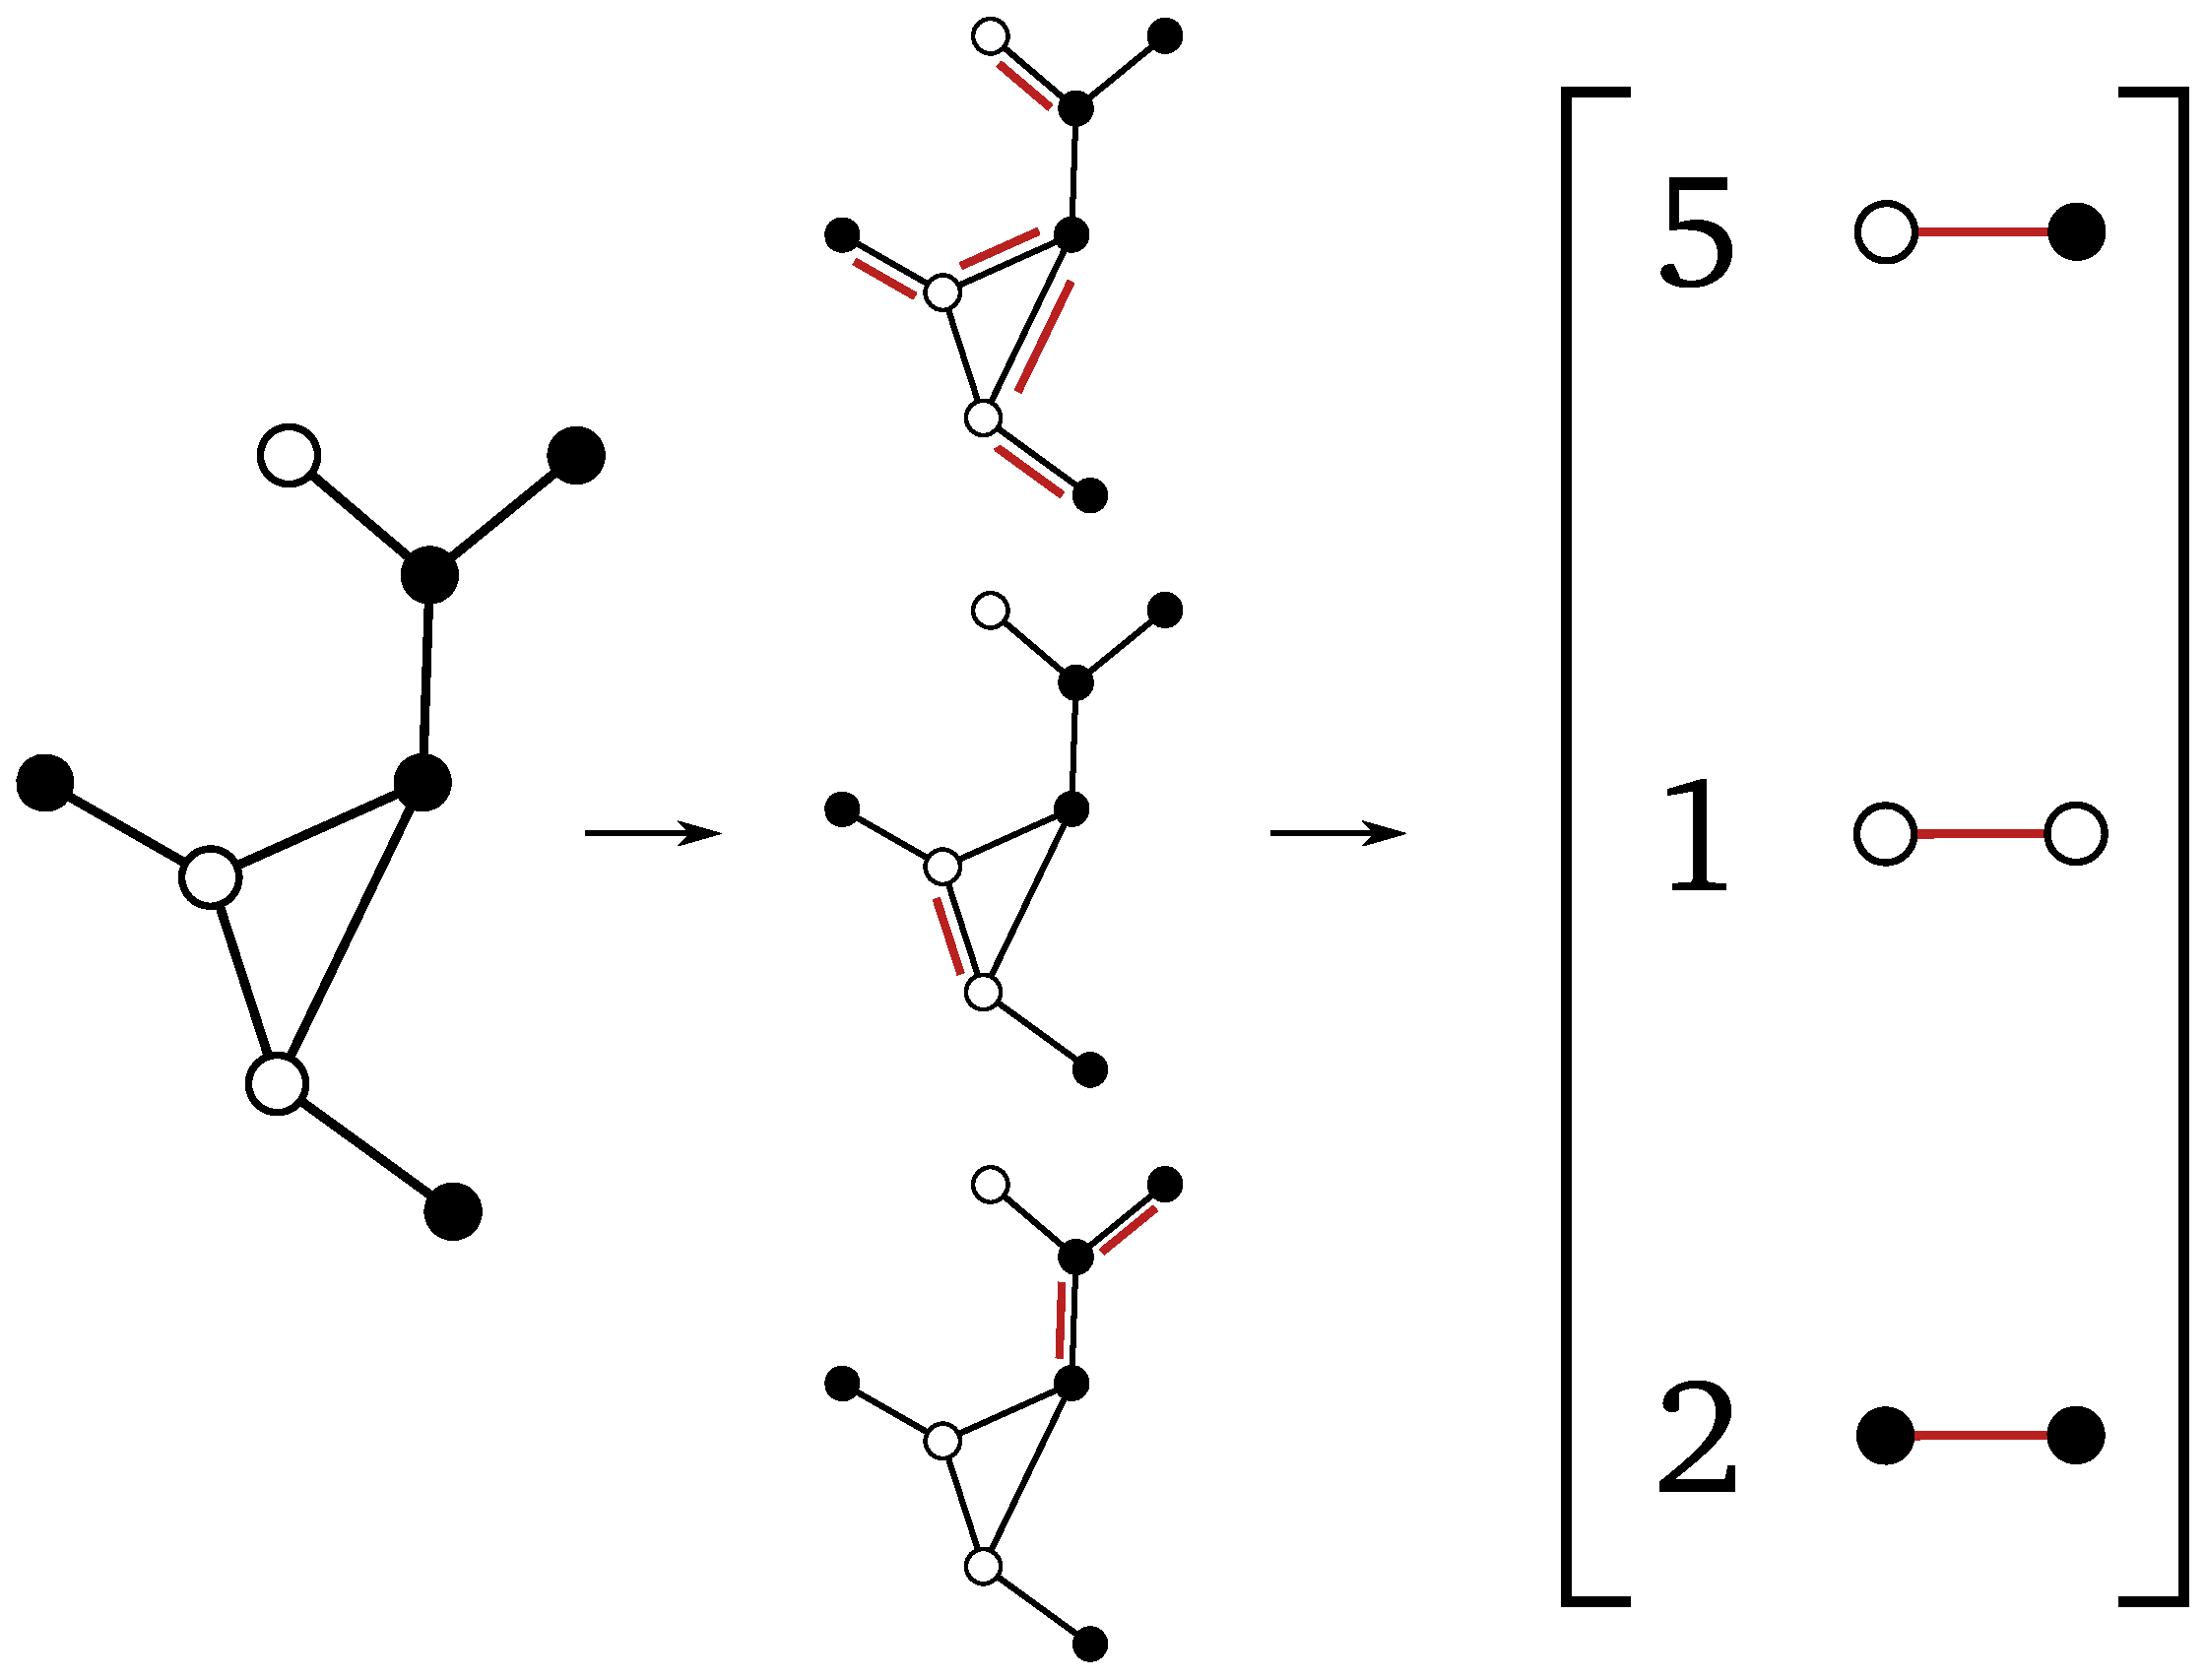
\includegraphics[width=0.9\textwidth]{subgraph-counting-labeled}
\caption{Illustration of the subgraph-enumeration process with a
  labeled input graph. In this case, we must discriminate between
  differently labeled subgraphs. \label{fig:sis5}}
\end{figure}

\section{An unlabeled graph example: the Watts-Strogatz model}

To validate the applicability of the above approach/graph similarity
measure on graph objects, we used the Watts-Strogatz (WS) network
generation model to construct a graph object dataset on which to apply
DMAPS. For a fixed graph size, the WS model relies on two parameters
to generate a so-called small-world network output
\cite{watts_collective_1998}. The first parameter $p$ is initially
used to generate a two-dimensional lattice where each vertex is
connected to all of its neighbors situated a distance at most $p$
away. For each vertex in the graph, we choose the edge that connects
it to its nearest neighbor and, with probability $r$, rewire this edge
to connect with a vertex chosen uniformly at random from the
graph. This procedure is repeated, each time considering the edge that
connects the next closest neighbor to the vertex in question until all
edges have been considered once, with no duplicate edges allowed. The
resulting graph is considered the output of the model. The networks
produced by this model exhibit various qualitatively different
properties as its “generating parameters” vary. For $r=1$ the model
reduces to generating an Erdős–Rényi random graph $G(n,p)$: a graph of
size $n$ for which the probability that any two vertices are connected
is $p$. On the other hand, for $r=0$ the graph remains a regular
lattice, with no random changes in its topology. Lastly, for
intermediate values of $r$ we get many local connections between
adjacent nodes and few edges between far away nodes, which is a
defining characteristic of small-world networks. These different
regimes are depicted in Figure~\ref{fig:sis6a}.

The WS algorithm was used to generate $n=2000$ different small-world
graphs, each with $n=100$ vertices. For each such graph
$G_i(p_i, r_i)$, we generated uniformly at random the two variables
$r_i ~ \mathrm{unif}[0,1]$ and $p_i ~ \mathrm{unif}[0,1]$. We thus are
confident that, by construction, this is a two-parameter set of graph
data, parametrized by the generating parameters $p$ and $r$. The
diffusion map embedding was then constructed by using the graph
similarity measure defined above. It was found that the first two
principal DMAP eigenvectors $\phi_2$ and $\phi_3$ were sufficient to
represent the data. This is confirmed by the two dimensional nature of
the $(\phi_2, \phi_3)$ manifold, shown in Figure~\ref{fig:sis6bc}
colored by $\log(r)$ and $p$. When considering the values of $p_i$ and
$r_i$ of the various data points (the various graphs) that lie on this
two-dimensional manifold, it can be observed that they vary in
directions visually independent of each other. This strongly suggests
that the transformation $f:(\phi_2, \phi_3) \rightarrow (r,p)$ has a
nonsingular Jacobian matrix, which in turn implies that the
transformation is bijective - the two variable pairs are one-to-one
with each other, and they each constitute coordinates of the network
dataset. This means that DMAPS discovered a reparameterization of the
two variables $r$ and $p$, which in this case were known in advance to
be (by construction) the variables that define this dataset. This
serves as a validation for the DMAPS approach and the chosen graph
similarity measure since, by only examining a dataset generated by the
WS model, the technique was able to “learn” that only two features
mattered, and that the two features were one-to-one with the
construction parameters $(r, p)$ that here were a priori known.


\begin{figure}[!htp]
\centering
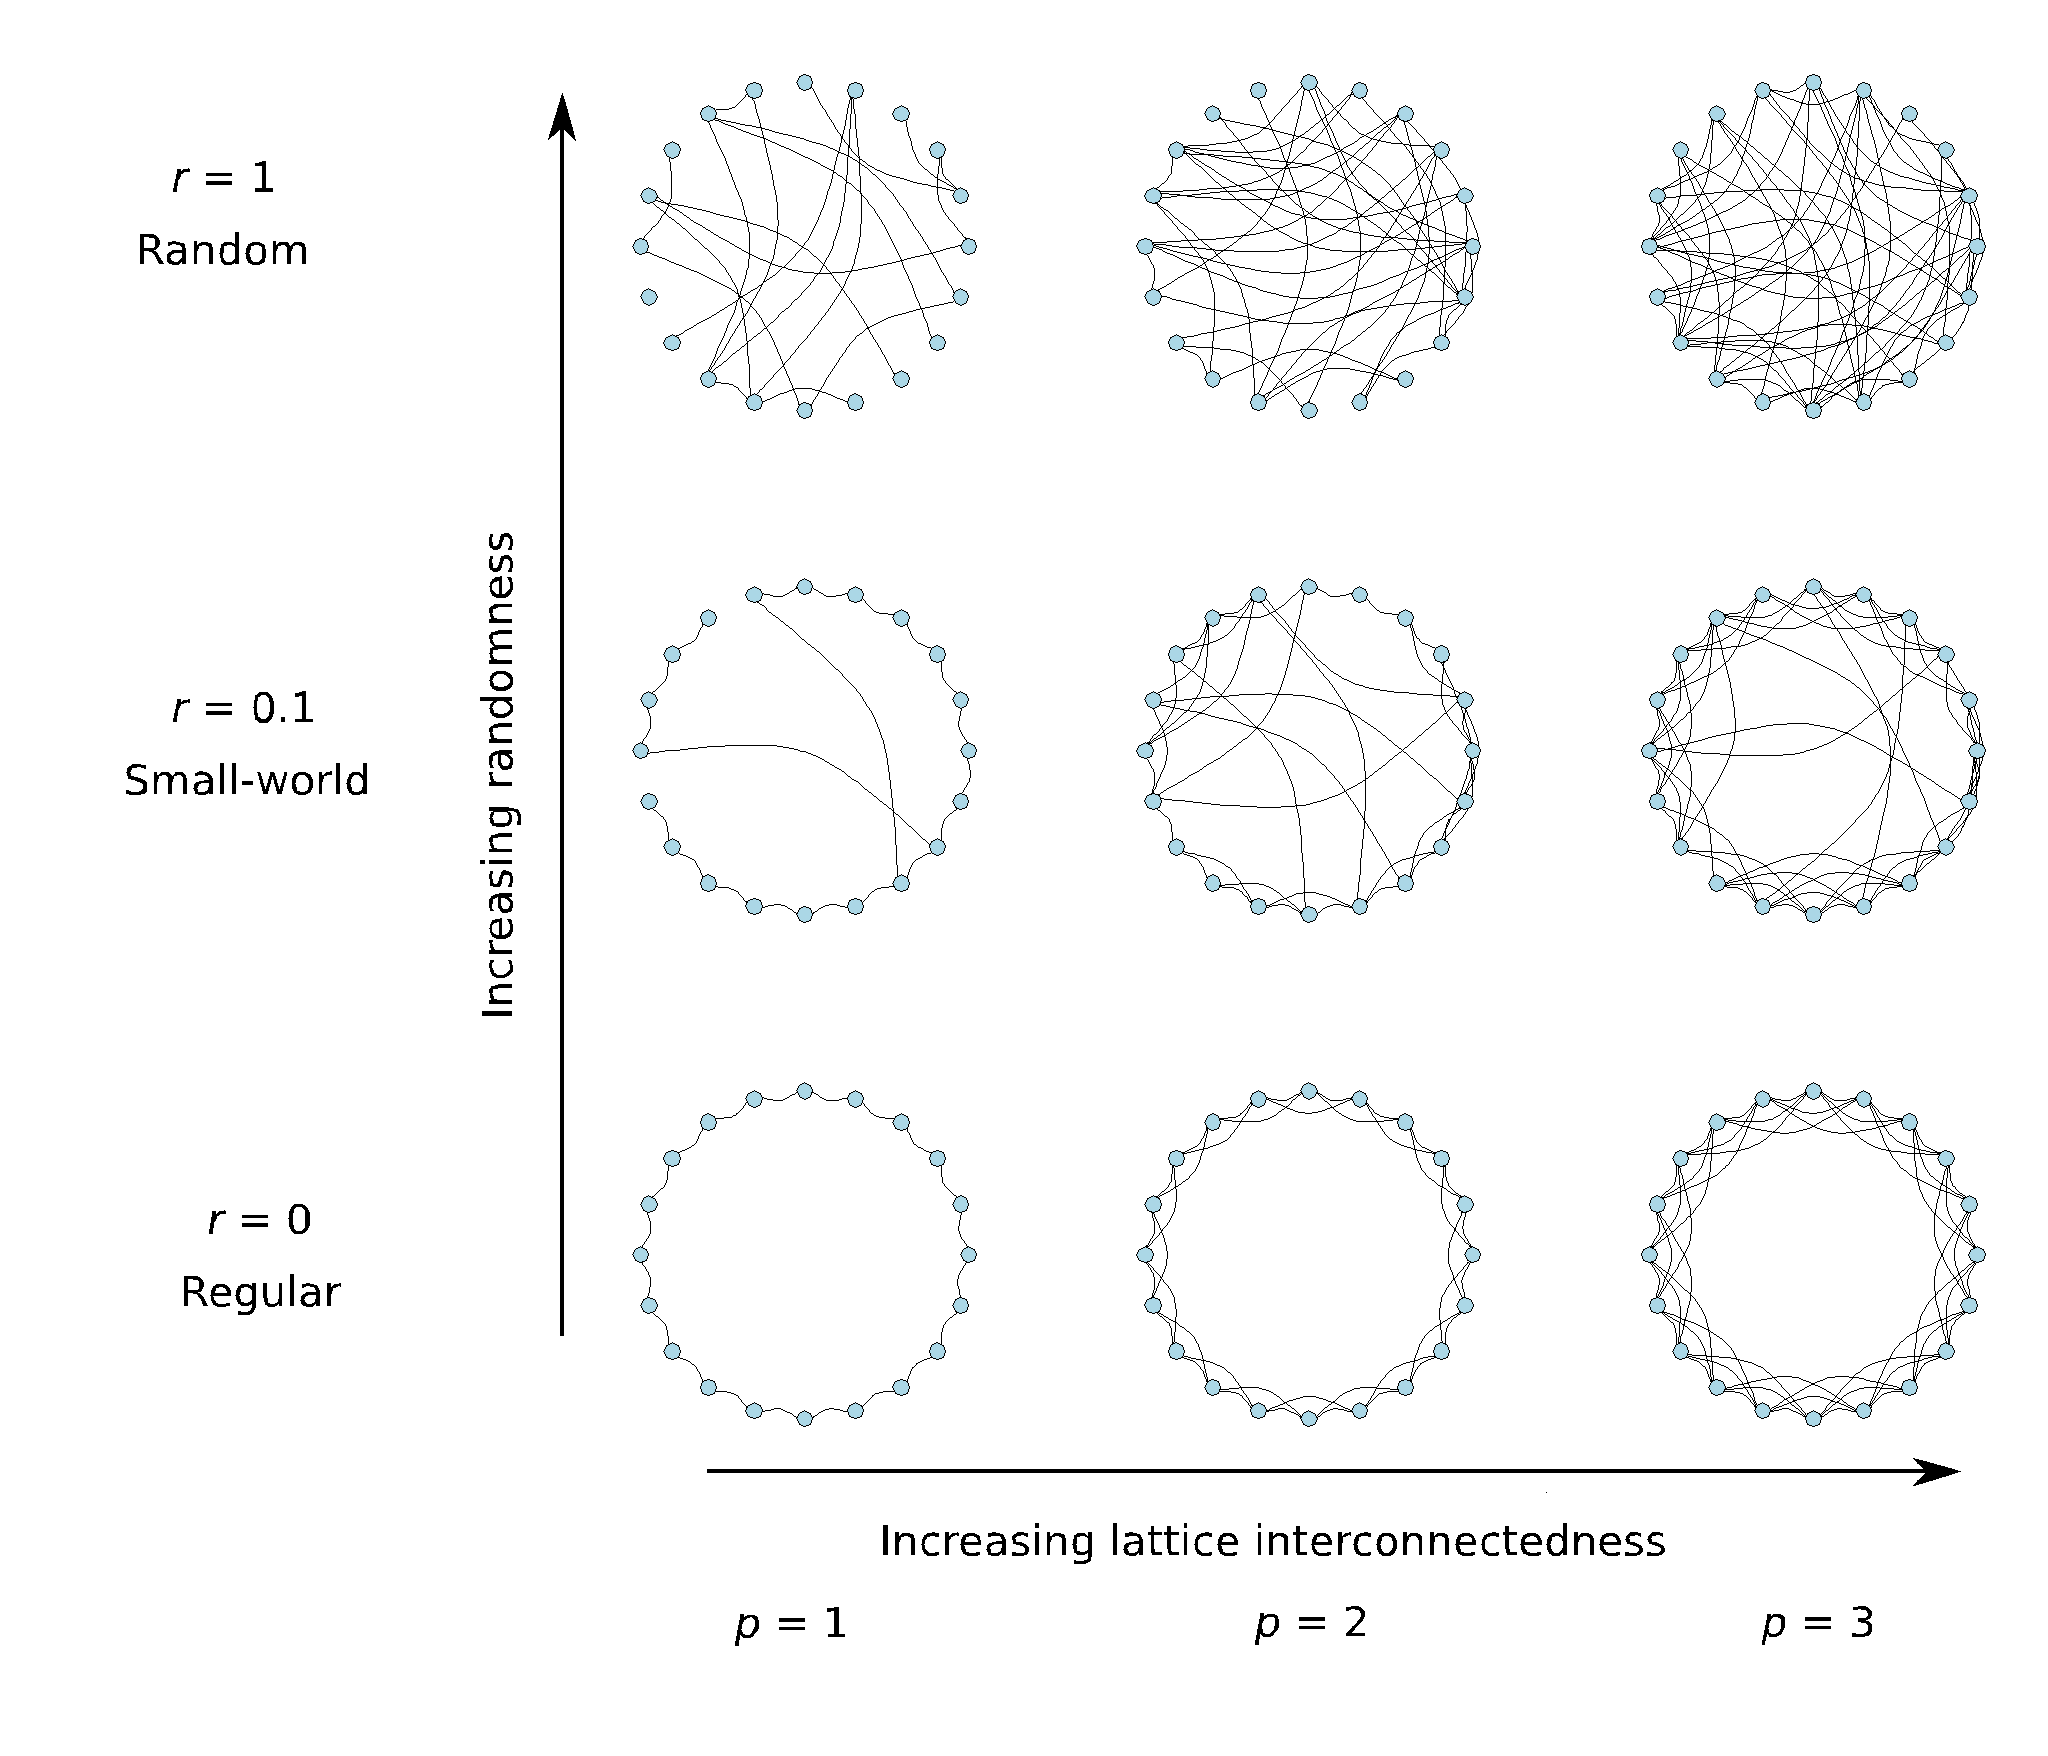
\includegraphics[width=0.9\textwidth]{6a}
\caption{The Watts-Strogatz Model and its construction parameters:
  The value of $r$ denotes the probability of long-distance rewiring
  with $r = 0$ denoting a regular lattice, $r < 1$ a small-world graph,
  and $r = 1$ an Erdős–Rényi random graph. The value of $p$ quantifies how
  interconnected the initial lattice is, being the number of
  neighboring nodes each node connects to. \label{fig:sis6a}}
\end{figure}

\begin{figure}[!htp]
\centering
\begin{tabular}{cc}
  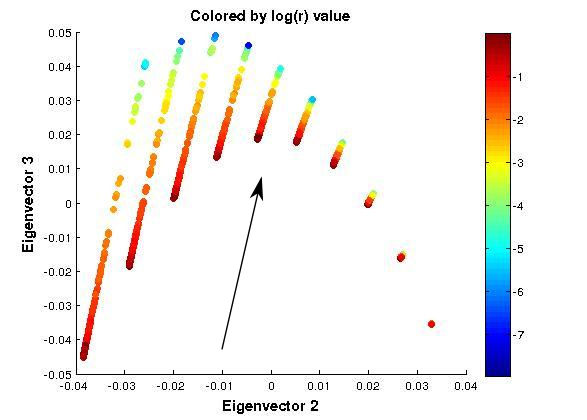
\includegraphics[width=0.45\textwidth]{6b} &
  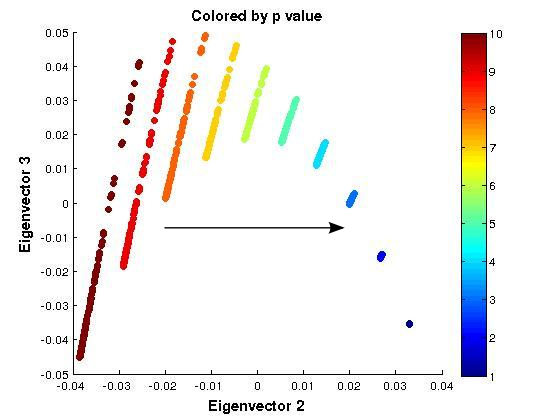
\includegraphics[width=0.45\textwidth]{6c}\\
  (a) & (b)
\end{tabular}
\caption{(a) Second versus third eigenvector $(\phi_2 ,\phi_3)$
  colored by $\log(r)$ (a) and $p$ (b). The visual linear independence
  of the directions of change of $\log(r)$ and $p$ indicate that the
  $(\phi_2 ,\phi_3)$ coordinates form a bijection with (a
  reparametrization of) the construction parameters $(r, p)$. An
  $\epsilon$ of 0.1 was used in our DMAPS
  computations. \label{fig:sis6bc}}
\end{figure}


\section{SIS model results}

In order to identify the coarse variables that parametrize the
dynamics of the adaptive SIS model, DMAPS were implemented on a graph
dataset sampled from the SIS model evolution. This dataset was
generated by systematically sampling graph objects from the SIS model
simulation over time from various parameters/initial conditions, with
each simulation leading to different long-term dynamical behavior. The
principal directions, represented by the leading diffusion map
coordinates, identify the important variables that define the model's
evolution over time. Since the set of coarse variables
$(i, l_{II}, l_{SS})$ are known to be central to the model's
evolution, their relationship with the derived principal directions
was investigated \cite{gross_robust_2008}.

More specifically, the system is known to undergo a Hopf bifurcation
to periodic solutions as the parameter $p$ varies around
$(p, r, w_0) \approx (0.00071, 0.0002, 0.06)$ and graph objects at
parameter values around this bifurcation point were sampled to create
a dataset of $N = 6000$ graphs ${G_i}_{i=1}^N$. After the graphs were
sampled, the DMAPS procedure detailed above was applied, with our
labeled graph metric used as a similarity measure. An analysis of the
relationship between the diffusion map coordinates indicates a
two-dimensional embedding in the first two principal directions
$\phi_2$, $\phi_3$, see Figures~\ref{fig:sis7} (a). Furthermore, an
investigation of the relationship between $\phi_2$ and $\phi_3$ with
other diffusion map coordinates demonstrates that no new direction is
captured by higher order eigenvectors, something that strongly implies
that the manifold on which the dataset lies is indeed
two-dimensional. This is achieved by performing linear regression,
with a suitable kernel, on the eigenvectors and checking whether each
can be accurately reconstructed using the rest, quantified as
cross-validation error, shown in Figures~\ref{fig:sis7} (b). This
measure is high for eigenvectors characterized by unique directions,
and low for higher harmonics and noise. It has the added benefit that
it can be used to compare many eigenvectors, not limiting it only to
the first few.

Motivated by the evidence that the $(\phi_2 ,\phi_3)$ manifold fully
captures all independent directions in the dataset, we look at the
relationship between these two principal directions and the coarse
variables $(i, l_{II}, l_{SS})$ , known to encapsulate the long-term
dynamics of this system. The relationship between $(\phi_2 ,\phi_3)$
and $(i, l_{II}, l_{SS})$ can be investigated by visually studying the
embedding of the coarse variables in diffusion map space. Looking at
the relationship between these three variables in our dataset, it can
be noticed that they actually span two (and not three different)
dimensions, which can be garnered by their two dimensional embedding
in $\mathbb{R}^3$. Thus, we are actually looking for two principal
directions, motivating the definition of
$l_{SI} = L − (l_{II} + l_{SS})$, the total number of SI-links as a
compound variable. This is done without introducing or removing any
information from the system, as the total number of edges is
11constant throughout. We consider $\log(l_{SI})$ as a candidate
macro-variable, since we are interested in finding a bijective
relationship between $(\phi_2 ,\phi_3)$ and $(i, l_{II}, l_{SS})$.

By inspecting the relative directions of $i$ and $\log(l_{SI})$ in the
two dimensional embedding of $(\phi_2 ,\phi_3)$, as shown in
Figure~\ref{fig:sis7} (c) and (d), it becomes apparent that they are
transverse to each other, with the former varying roughly from left to
right and the latter from top to bottom. Such an observation is strong
evidence that the Jacobian of the transformation
$f:(\phi_2, \phi_3) \rightarrow (i, l_{SI})$ is nonsingular on this
dataset, much in the same manner as for the Watts-Strogatz graph
ensembles. Thus, we can conclude that the directions of change on the
$(\phi_2 ,\phi_3)$ manifold represented by changing $i$ and $l_{SI}$,
respectively, are independent of each other, and that they are
reparametrizations of the principal eigenvectors. Similar results are
obtained if we consider $l_{SI}$ instead of $\log(l_{SI})$. These
observations imply that the diffusion map technique has been
successful in identifying, up to parameterization, the variables found
in ~\cite{gross_robust_2008} as responsible for the long term dynamics
of the model. Furthermore, we were able to confirm that the long-term
dynamics of this model really depend on only two macro-variables, the
total number of infected nodes $i$ and the total number of SI-links
$l_{SI}$. Figures~\ref{fig:sis7} (e) and (f) show other colorings of
the $(\phi_2 ,\phi_3)$ plane, and Figure~\ref{fig:sis8} shows the
two-dimensional nature of the system as seen in three dimensions.

In addition, there was no need to take any a priori knowledge about
the model's specifics into account when isolating the important
variables. Instead, we required the development of a suitable
similarity measure between labeled graphs, which can be generalized
for use with other problems (models, datasets) that exhibit completely
different dynamic behavior. This generalization of feature extraction
for high-dimensional systems can assist in developing a framework for
isolating the coarse variables that define graph-based datasets
without resorting to approaches that rely on intuition about the
specific model.


\begin{figure}[!htp]
\centering
\begin{tabular}{cc}
  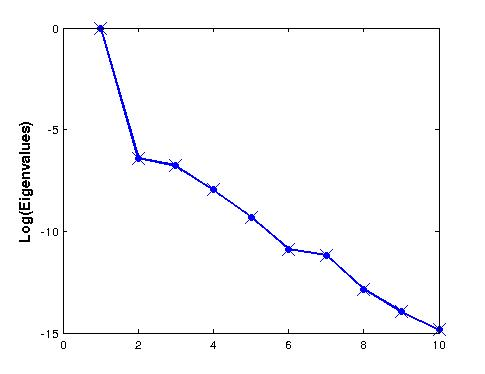
\includegraphics[width=0.45\textwidth]{7a} &
  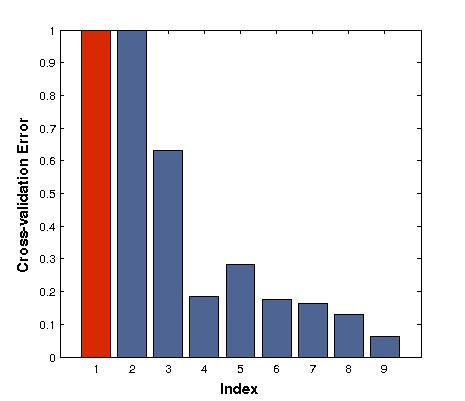
\includegraphics[width=0.45\textwidth]{7b}\\
  (a) & (b)\\
  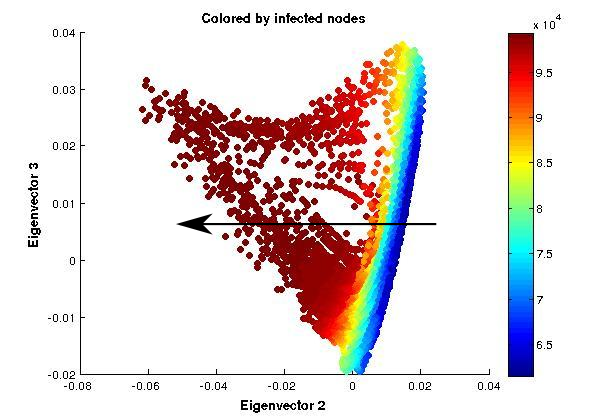
\includegraphics[width=0.45\textwidth]{7c} &
  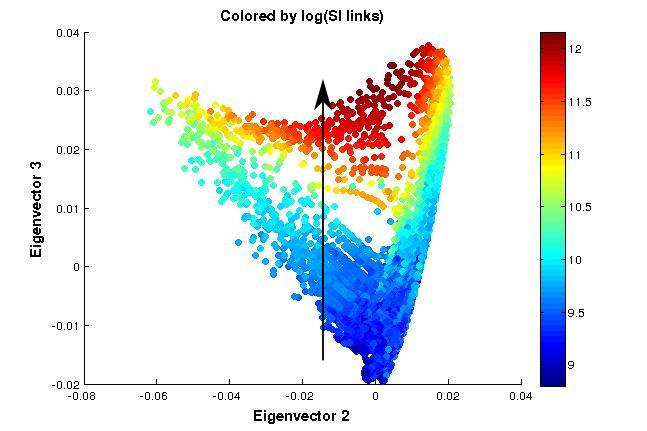
\includegraphics[width=0.45\textwidth]{7d}\\
  (c) & (d)\\
  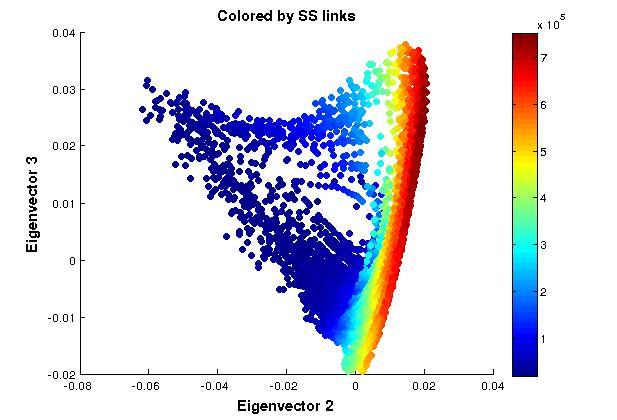
\includegraphics[width=0.45\textwidth]{7e} &
  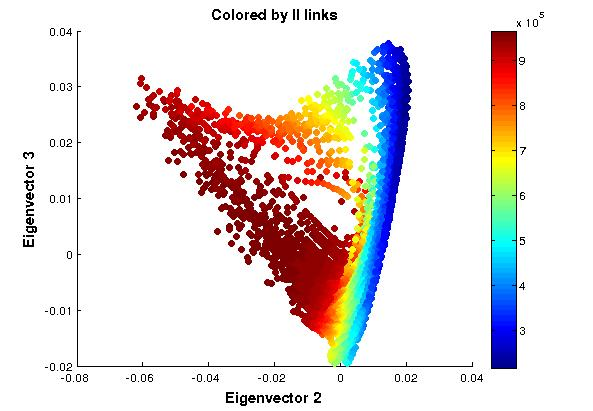
\includegraphics[width=0.45\textwidth]{7f}\\
  (e) & (f)
\end{tabular}
\caption{Coarse variable detection: (a) The leading eigenvalues of the
  random walk matrix are plotted. (b) Computation a criterion
  suggesting that the first two eigendirections suffice (the first is
  a trivial one, and the third is much less important than the first
  two. The $x$ and $y$ coordinates of the middle and bottom row
  figures indicate the components of each datum, representing a graph,
  in the second and third eigenvectors of the random walk matrix. Each
  point is also colored by the number of (c) infected nodes $i$, (d)
  $\log$(SI-links), (e) SS-links, and (f) II-links found in the
  corresponding graph. A comparison between (c) and (d) indicates a
  linear independence relationship between $i$ and $log(l_{SI})$. An
  $\epsilon$ of 70 was used. \label{fig:sis7}}
\end{figure}

\begin{figure}[!htp]
\centering
\begin{tabular}{cc}
  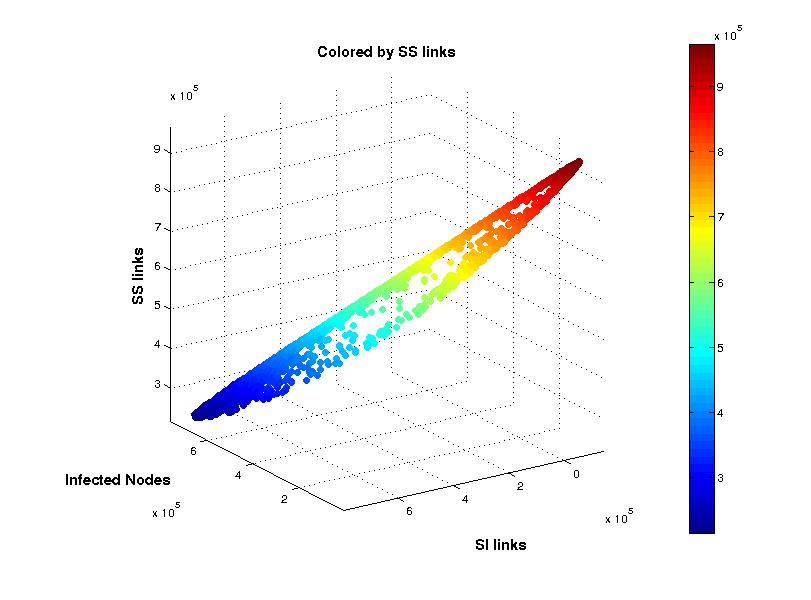
\includegraphics[width=0.45\textwidth]{8a} &
  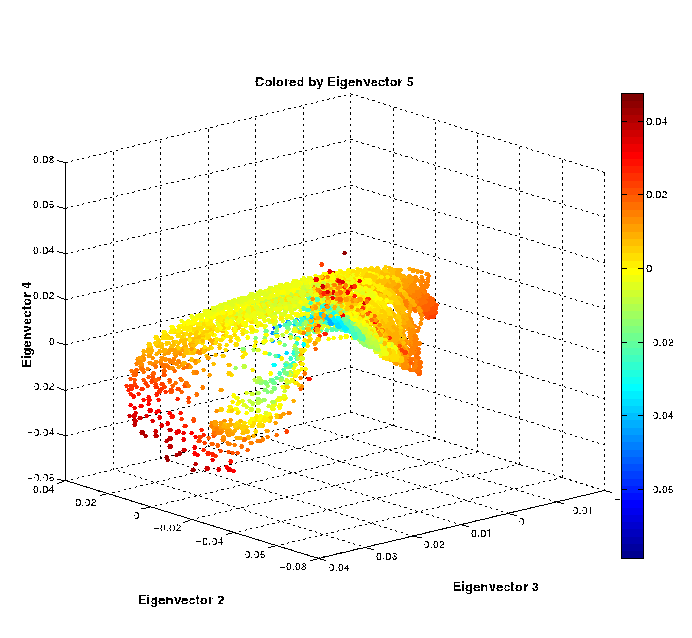
\includegraphics[width=0.45\textwidth]{8b}\\
  (a) & (b)
\end{tabular}
\caption{Coarse Variable Dependencies: An illustration of the
  relationship between $l_{SS}$, $l_{SI}$, and $i$ in the diffusion
  map dataset. The two-dimensional nature of the manifold indicates
  that the number of SS links can be thought of as a function, on the
  data, of $i$ and $l_{SI}$, and is thus not necessary as an
  independent macro-variable. \label{fig:sis8}}
\end{figure}


\section{Conclusion}

The use of networks in the modeling of real-world phenomena is
particularly suited to modeling the spread of an epidemic through a
population represented as a network of geographic/social
connections. In this paper, the suitability of data mining techniques
for extracting the important macro-variables describing the evolution
of network connectivity from an adaptive SIS model were investigated,
based on two concepts. Firstly, a dissimilarity metric for graph
objects was constructed; secondly, it was used with the DMAPS
nonlinear data-mining procedure. In particular, we needed to define a
(dis)similarity measure between different labeled graphs, as they
arise in the course of the epidemic model simulation. It should be
noted that this method is generalizable to any labeled graph with
distinct labels, and can be utilized regardless of the overarching
process defining graph evolution. Future work in this area should
investigate the suitability of other graph similarity measures for use
within the DMAPS framework. Moreover, this approach is not DMAPS-
specific. Indeed, other non-linear data mining techniques are expected
to yield similar results, provided they use the aforementioned
dissimilarity measure.

In addition, the long-term dynamics of a particular adaptive SIS model
were explored, which allowed us to verify the suitability of the
constructed metric for use with graph object datasets. This yields two
interconnected results. Firstly, the DMAP procedure was able to
demonstrate that the system is inherently macroscopically two
dimensional, with the two independent directions in the dataset being
represented by the first two nontrivial Diffusion Map
eigenvectors. This result is consistent with previous knowledge about
the dimensionality of the model’s dynamics, and is strong evidence
that the DMAP framework, using the similarity measure we constructed,
can be readily applied to graph object data sets to extract meaningful
reduced parametrizations of the underlying behavior.

Furthermore, we were also able to link the principal diffusion map
coordinates with previously known coarse variables capable of
describing this system. By inspection of the embeddings in diffusion
space, it was verified that a bijection exists between two of these
coarse variables and the two leading diffusion map coordinates. This
means that the DMAP was not only able to learn the inherent
dimensionality of the dataset, but that it was also able to extract a
reparameterization of variables known to fully specify this model;
what is unfortunate, is that the variables of this reparametrization
have no obvious unique, easily explainable physical meaning.

This modeling exercise clearly shows that modern data mining
techniques for data in the form of high-dimensional evolving vectors
can be extended to data in the form of large evolving graphs (labeled
or unlabeled). This holds promise for the analysis of data from
epidemics on realistic adaptive networks, and for general adaptive
network evolution problems. What is more important and more promising,
however, is that these data-based coarse descriptors can be used, in
an equation-free framework, to implement accurate reduced model
computations for the epidemic dynamics, in which the variables used to
describe the systems-level network behavior are the ones obtained from
data mining. This data-driven model reduction approach can be
introduced as a “wrapper algorithm” around brief bursts of detailed,
fine scale simulation; we believe that the approach holds real promise
in enabling systems level analysis, simulation and control of
detailed, realistic epidemic dynamics.

We have now seen two unique applications of DMAPS to network
systems. The next chapter will again employ this nonlinear manifold
learning technique, but in a different application. We will see how
DMAPS can be used to uncover important parameter combinations in
systems of differential equations.



%%% Local Variables: ***
%%% mode:latex ***
%%% TeX-master: "../../thesis.tex"  ***
%%% End: ***